\section{Contexte de développement}

Avant de réaliser une planification de notre travail pour les mois à venir, il convenait d'établir le contexte de notre projet, c'est à dire le cahier des charges que nous avons à remplir et  les effectifs dont nous disposerons.

\subsection{Cahier des charges}

Le projet Avalon a été proposé à l'initiative du centre de rééducation de Kerpape dans et a pour finalité d'être utilisé dans le cadre des soins qu'ils fournissent à leurs patients. Cela est un point important pour nous car il s'agit d'un client extérieur à l'INSA, et donc d'une expérience proche de celle que l'on pourrait rencontrer en entreprise. \newline

Nous avons longuement discuté avec Willy Allègre et Jean-Paul Departe, les ingénieurs de Kerpape avec qui nous sommes en relation, pour établir notre cahier des charges. Celui-ci a été longuement détaillé dans le rapport de pré-étude, nous en donnerons ici une version résumée qui reprend l'essence des attentes de nos commanditaires. 

\subsubsection{Trois modes de fonctionnement}

\textbf{Apprentissage symbolique}
\newline
Ce mode doit permettre de tout apprendre depuis le début et de comprendre le fonctionnement global des différentes situations auxquelles l'utilisateur peut être confronté. Il comporte des vues statiques, \enquote{zoomées}, avec la mise en évidence d'actions à réaliser, ainsi que des indications visuelles symboliques.\newline

\textbf{Assisté}
\newline
Dans un environnement réaliste, le logiciel donne des indications légères pour permettre de retrouver les actions à faire. Ces indications sont activables par les ergothérapeutes. Par exemple :
\begin{itemize}
  \item la surbrillance des objets à actionner,
  \item lors de l'activation d'une action on accède à une vue fixe avec les états courants des équipements afin de faciliter la compréhension du lien action/objet pour l'utilisateur. \newline
\end{itemize}

\textbf{Autonome}
\newline
L'utilisateur ne reçoit plus d'information ou d'indication pour effectuer son parcours, il est dans le décor le plus réaliste possible, pour valider son autonomie. Il doit alors actionner les différents objets et se rendre compte par lui même (déplacement) des actions qu'il a effectuées.

\subsubsection{Deux points de vue}

\textbf{Exocentré}
\newline
Une vue à la troisième personne (exocentrée) permet de voir le déplacement de l'utilisateur dans la scène. Grâce à cette vue, l'utilisateur peut mieux voir les interactions avec son environnement et avoir une vision plus globale sur la scène. On peut ainsi avoir des angles de caméra qu'un avatar virtuel ne pourrait avoir ; il est par exemple possible de voir à la fois devant et derrière soi (cf.\textsc{figure~\ref{exo}}).

\textbf{Endocentré}
\newline
Une vue à la première personne (endocentrée) sera aussi incluse, permettant une immersion totale dans la scène. En effet, ce type de vision est proche du point de vue humain, ce qui permet une identification facile à l'avatar virtuel pour l'utilisateur. C'est donc le type de vue le plus logique en réalité virtuelle (cf. \textsc{figure~\ref{endo}}).

\begin{figure}[h]
	\centering
	\begin{minipage}[b]{0.3\textwidth}
		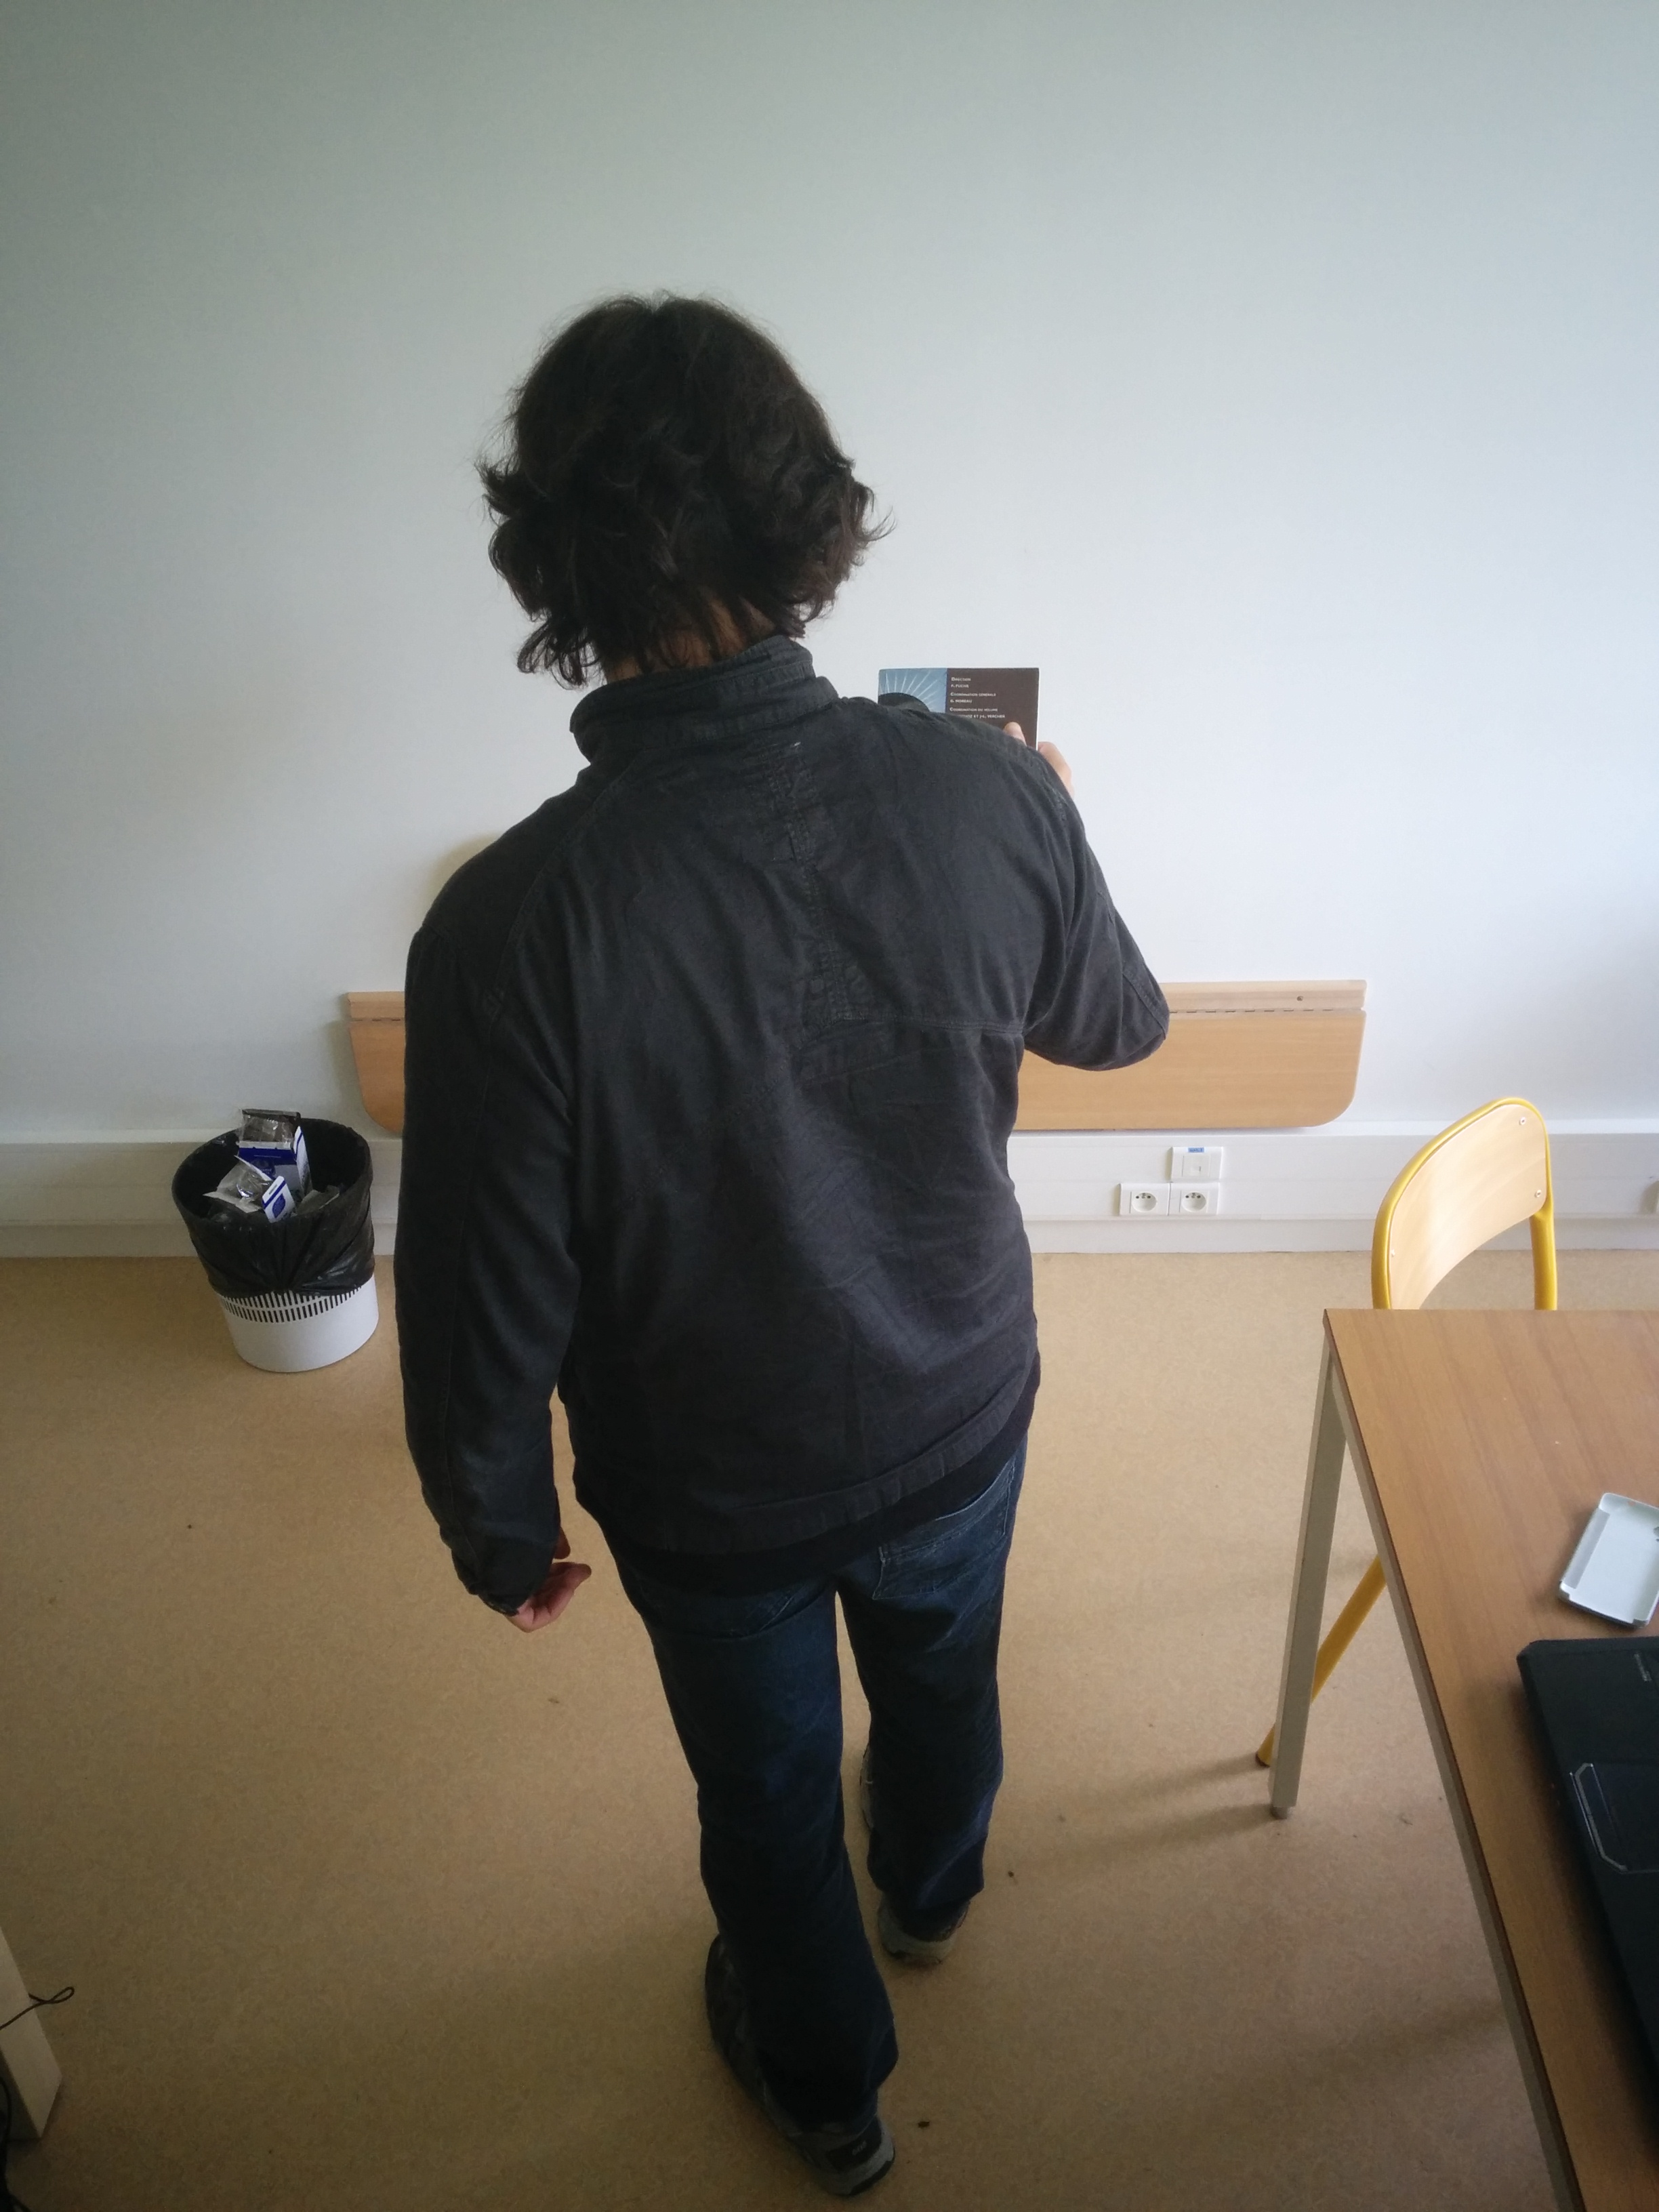
\includegraphics[width=\linewidth]{3-Planification/img-utilisateur/vue_tps}
		\caption{Vue exocentrée}
		\label{exo}
	\end{minipage}
	\begin{minipage}[b]{0.3\textwidth}
		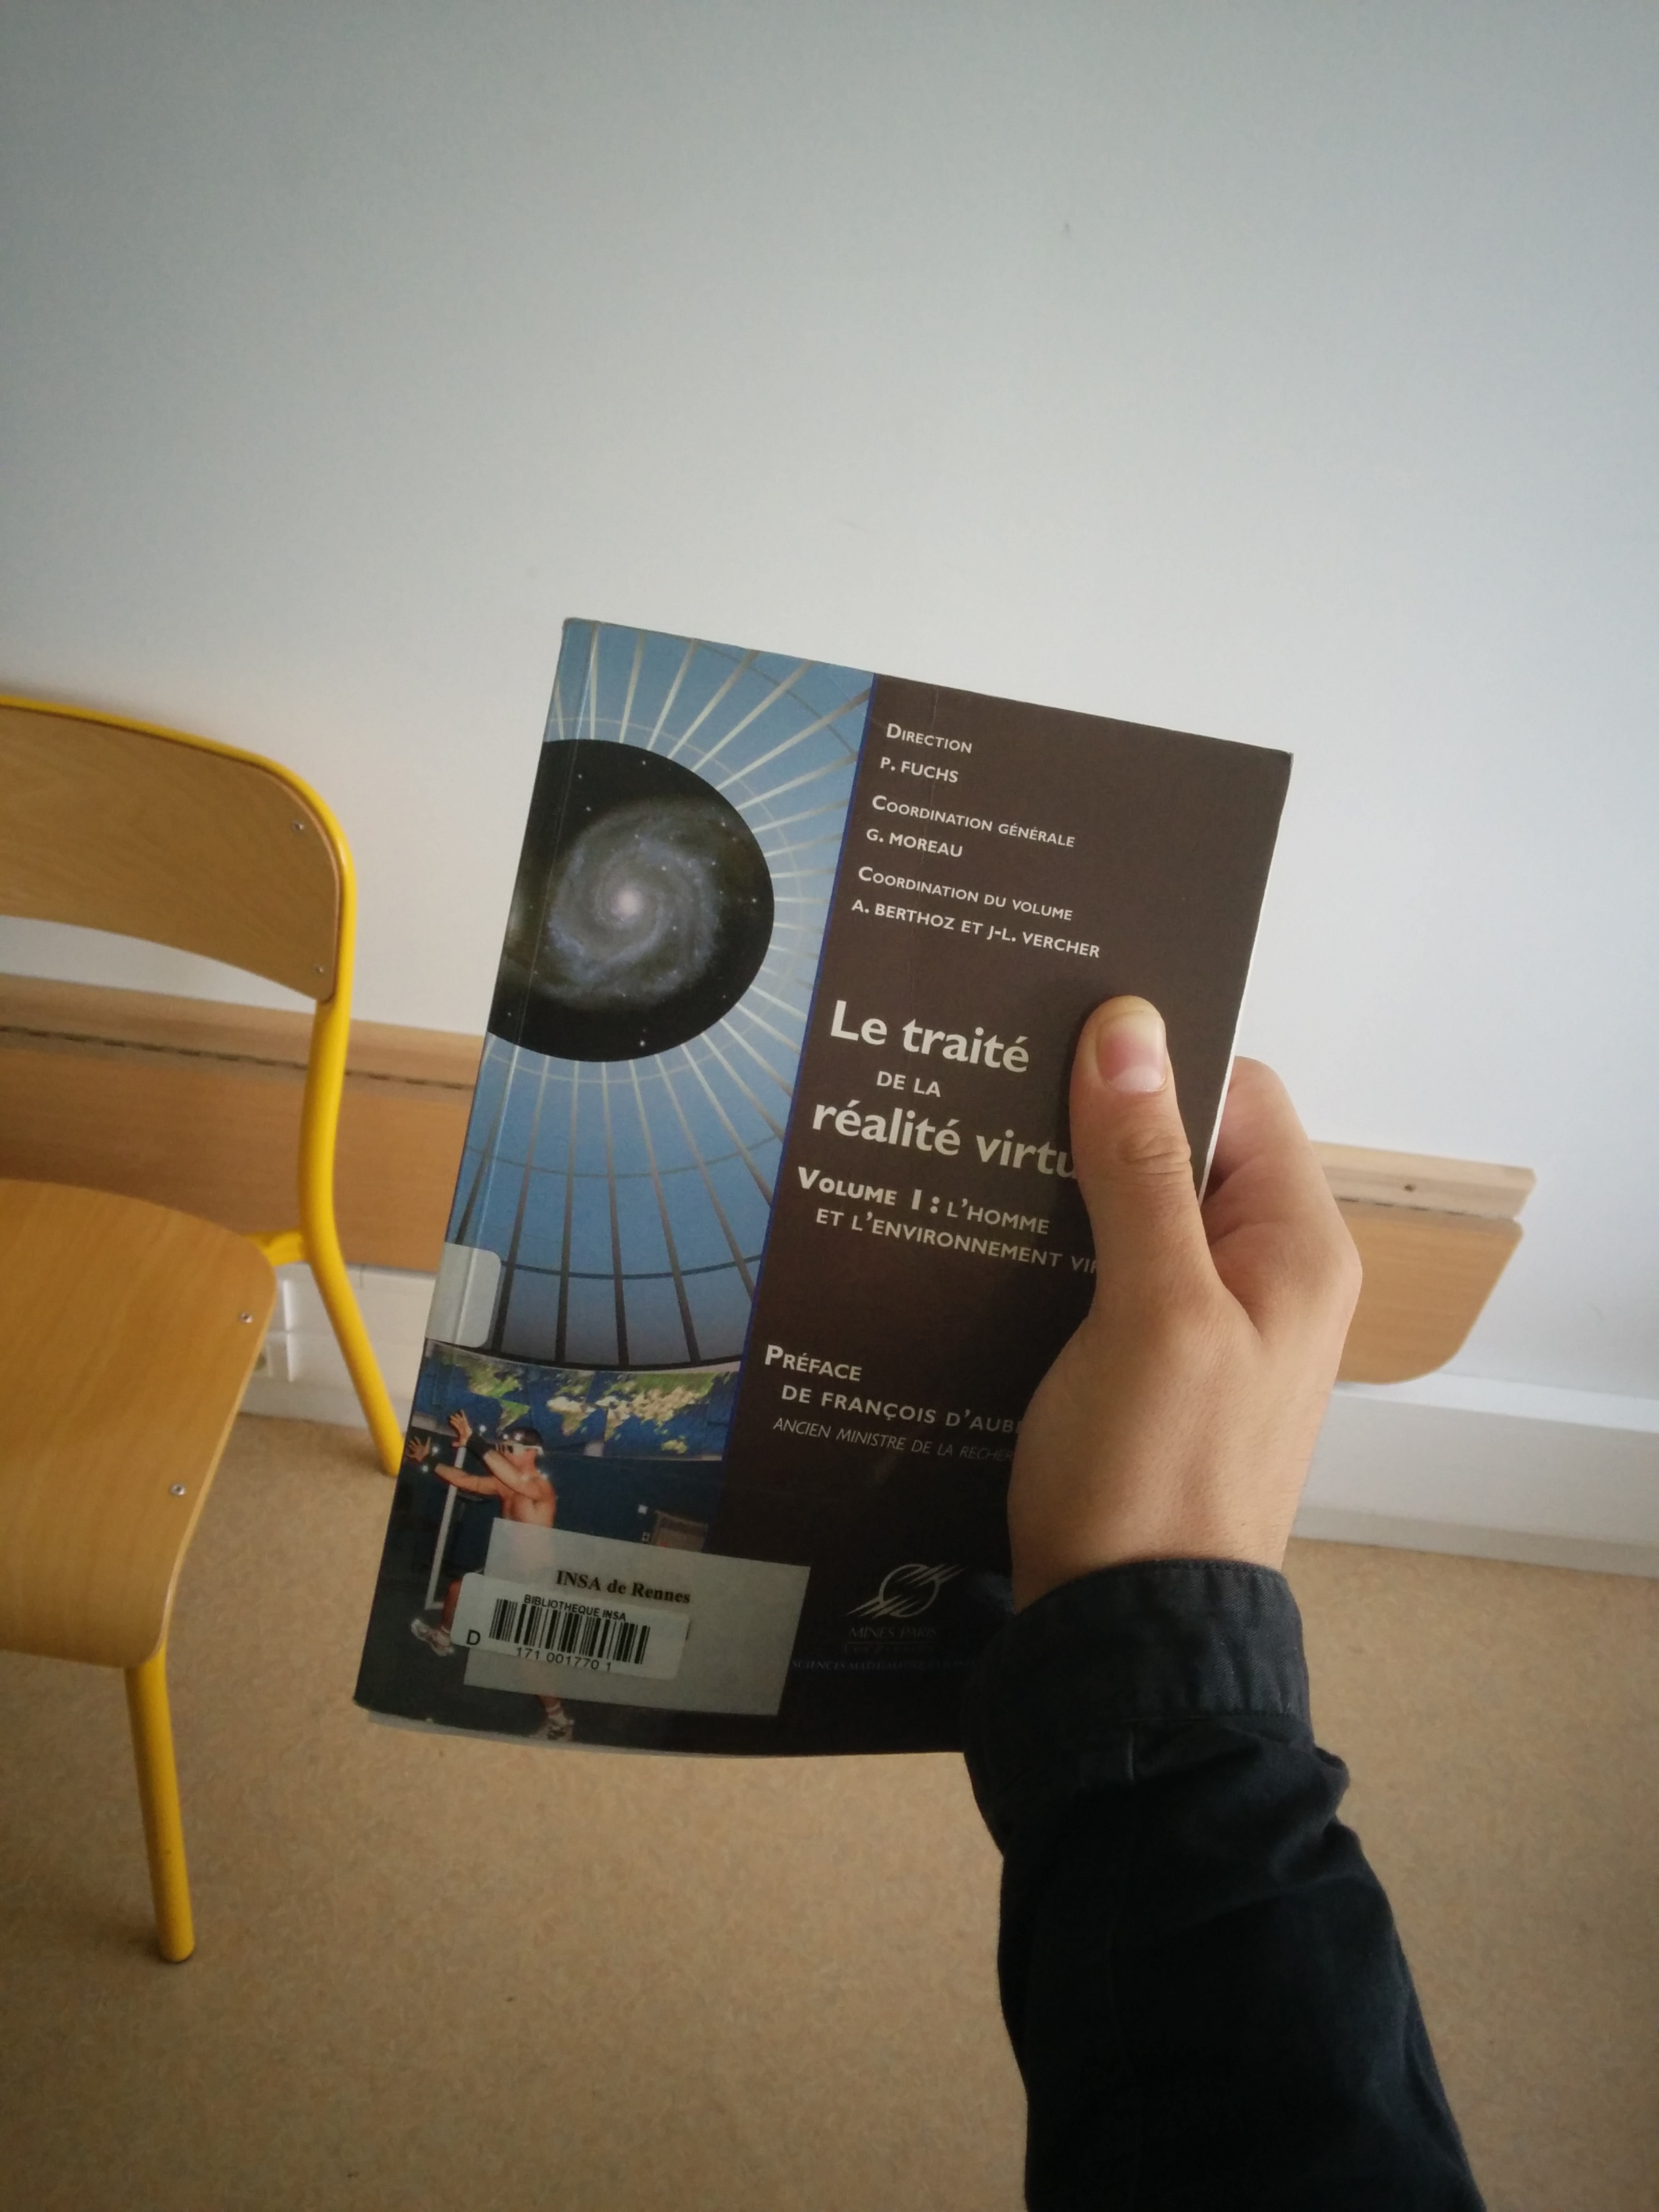
\includegraphics[width=\linewidth]{3-Planification/img-utilisateur/vue_fps}
		\caption{Vue endocentrée}
		\label{endo}
	\end{minipage}
\end{figure}

\subsubsection{Scénarios}
Trois scénarios autour de l'appel sur le téléphone sont à prévoir avec des actions différentes à entreprendre décrites dans l'étude fonctionnelle. \newline

\textbf{Appel téléphonique: }\emph{Appel téléphonique (d'un proche ou d'une personne qui se serait trompée de numéro). }
%- L'utilisateur doit pouvoir décrocher le téléphone pour entrer en communication puis raccrocher quand la communication est terminée.

\textbf{Interphone infirmier: } \emph{Appel venant du portier audio/vidéo sur le téléphone (d'un infirmier qui souhaiterait entrer). }
%L'utilisateur doit pouvoir décrocher le téléphone, communiquer avec l'infirmier, raccrocher le téléphone et ouvrir la porte.

\textbf{Interphone inconnu: } \emph{Appel venant du portier audio/vidéo sur le téléphone (d'un inconnu). }
%L'utilisateur doit pouvoir décrocher le téléphone pour entrer en communication, allumer la TV pour voir la vidéo puis éteindre la TV et raccrocher le téléphone à la fin de la conversation.